\chapter{Test Journal: DC motor moment of inertia $\boldsymbol{J_m}$}\label{appendix:TJDCMotorMomentofinertia}
\begin{table}[!h]
\begin{tabular}{l l}
\textbf{Test participants:} & Maxime, Robin \& Alexander\\
\textbf{Date:}  & 09/11-2016
\end{tabular}
\end{table}

\section*{Purpose}
The purpose of this test is to determine the moment of inertia of the motor's rotational body. This is done by applying voltage step to the DC motor and observing its dynamic properties.
\section*{Test equipment and components}
The test equipment and components are listed in \autoref{tab_appendix:testJm}.
\begin{table}[h]
	\centering
	\caption{List of measurement equipment and components}

	\begin{tabularx}{\textwidth}{lXXXX}
		Name 				& Brand	& Model & AAU-number\\ \toprule \rowcolor{lightGrey}
		Oscilloscope	& Agilient technologies & DSO6034A & 60763	\\
		Powersupply	& HP & E3631A & 78574\\ \rowcolor{lightGrey}
		DC motor & Maxon & 41.023.038-00.00-052& N/A \\ 
		Multimeter & Fluke & 37 & 33019\\\rowcolor{lightGrey}
		$\SI{1}{\ohm}$ resistor	& N/A & N/A & N/A
	\end{tabularx}
\end{table}\label{tab_appendix:testJm}
\section*{Setup}
A diagram of the setup to measure $J_m$ is illustrated on \autoref{Appendix:fig:DCMotorJmSetup}.

\begin{figure} [h]
    \centering
        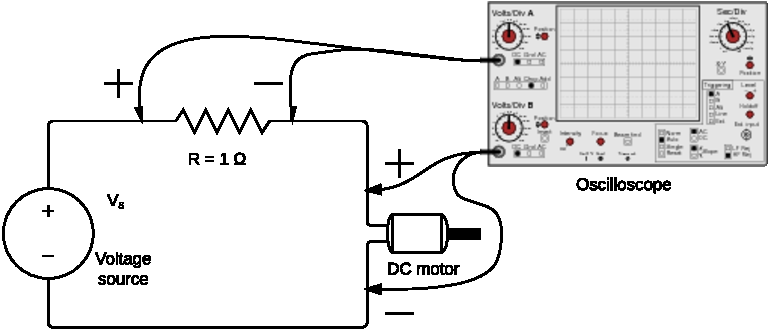
\includegraphics[width=\textwidth]{figures/test/DCTestJ}
        \caption{Diagram of the setup. Oscilloscope icon is from \cite{web:OscilloscopeIcon}}
        \label{Appendix:fig:DCMotorJmSetup}
\end{figure}

%$\approx$8 ms for voltage source to rise to 99\% (for 2 to 10 V)

\section*{Method}
The motor is connected to the resistor and the voltage source. The oscilloscope is connected to the measuring points as indicated on \autoref{Appendix:fig:DCMotorJmSetup}. A voltage step is applied to measure the step response, a moment of inertia that fits the dynamic properties of the motors rotational body can be determined. A step from \SI{2}{\volt} to \SI{10}{\volt} is applied, since the friction at an angular velocity of $\omega_m = 0$ is expected to be nonlinear. Therefore:
\begin{enumerate}
\item Set the voltage supply to \SI{2}{\volt}.
\item Wait for system to reach steady state.
\item Set the oscilloscope to trigger on the next rising slope.
\item Change the voltage supply to \SI{10}{\volt} in a single step.
\item Save the curve of the voltage and current from the oscilloscope.
\end{enumerate}

\section*{Results}
On \autoref{Appendix:fig:DCMotorMomentOfIntertia} the results from the test are illustrated. The current is calculated by using the voltage across the resistor $R=\SI{1}{\ohm}$ and Ohm's law $V = R \cdot I$.
\begin{figure}[!h]
\centering
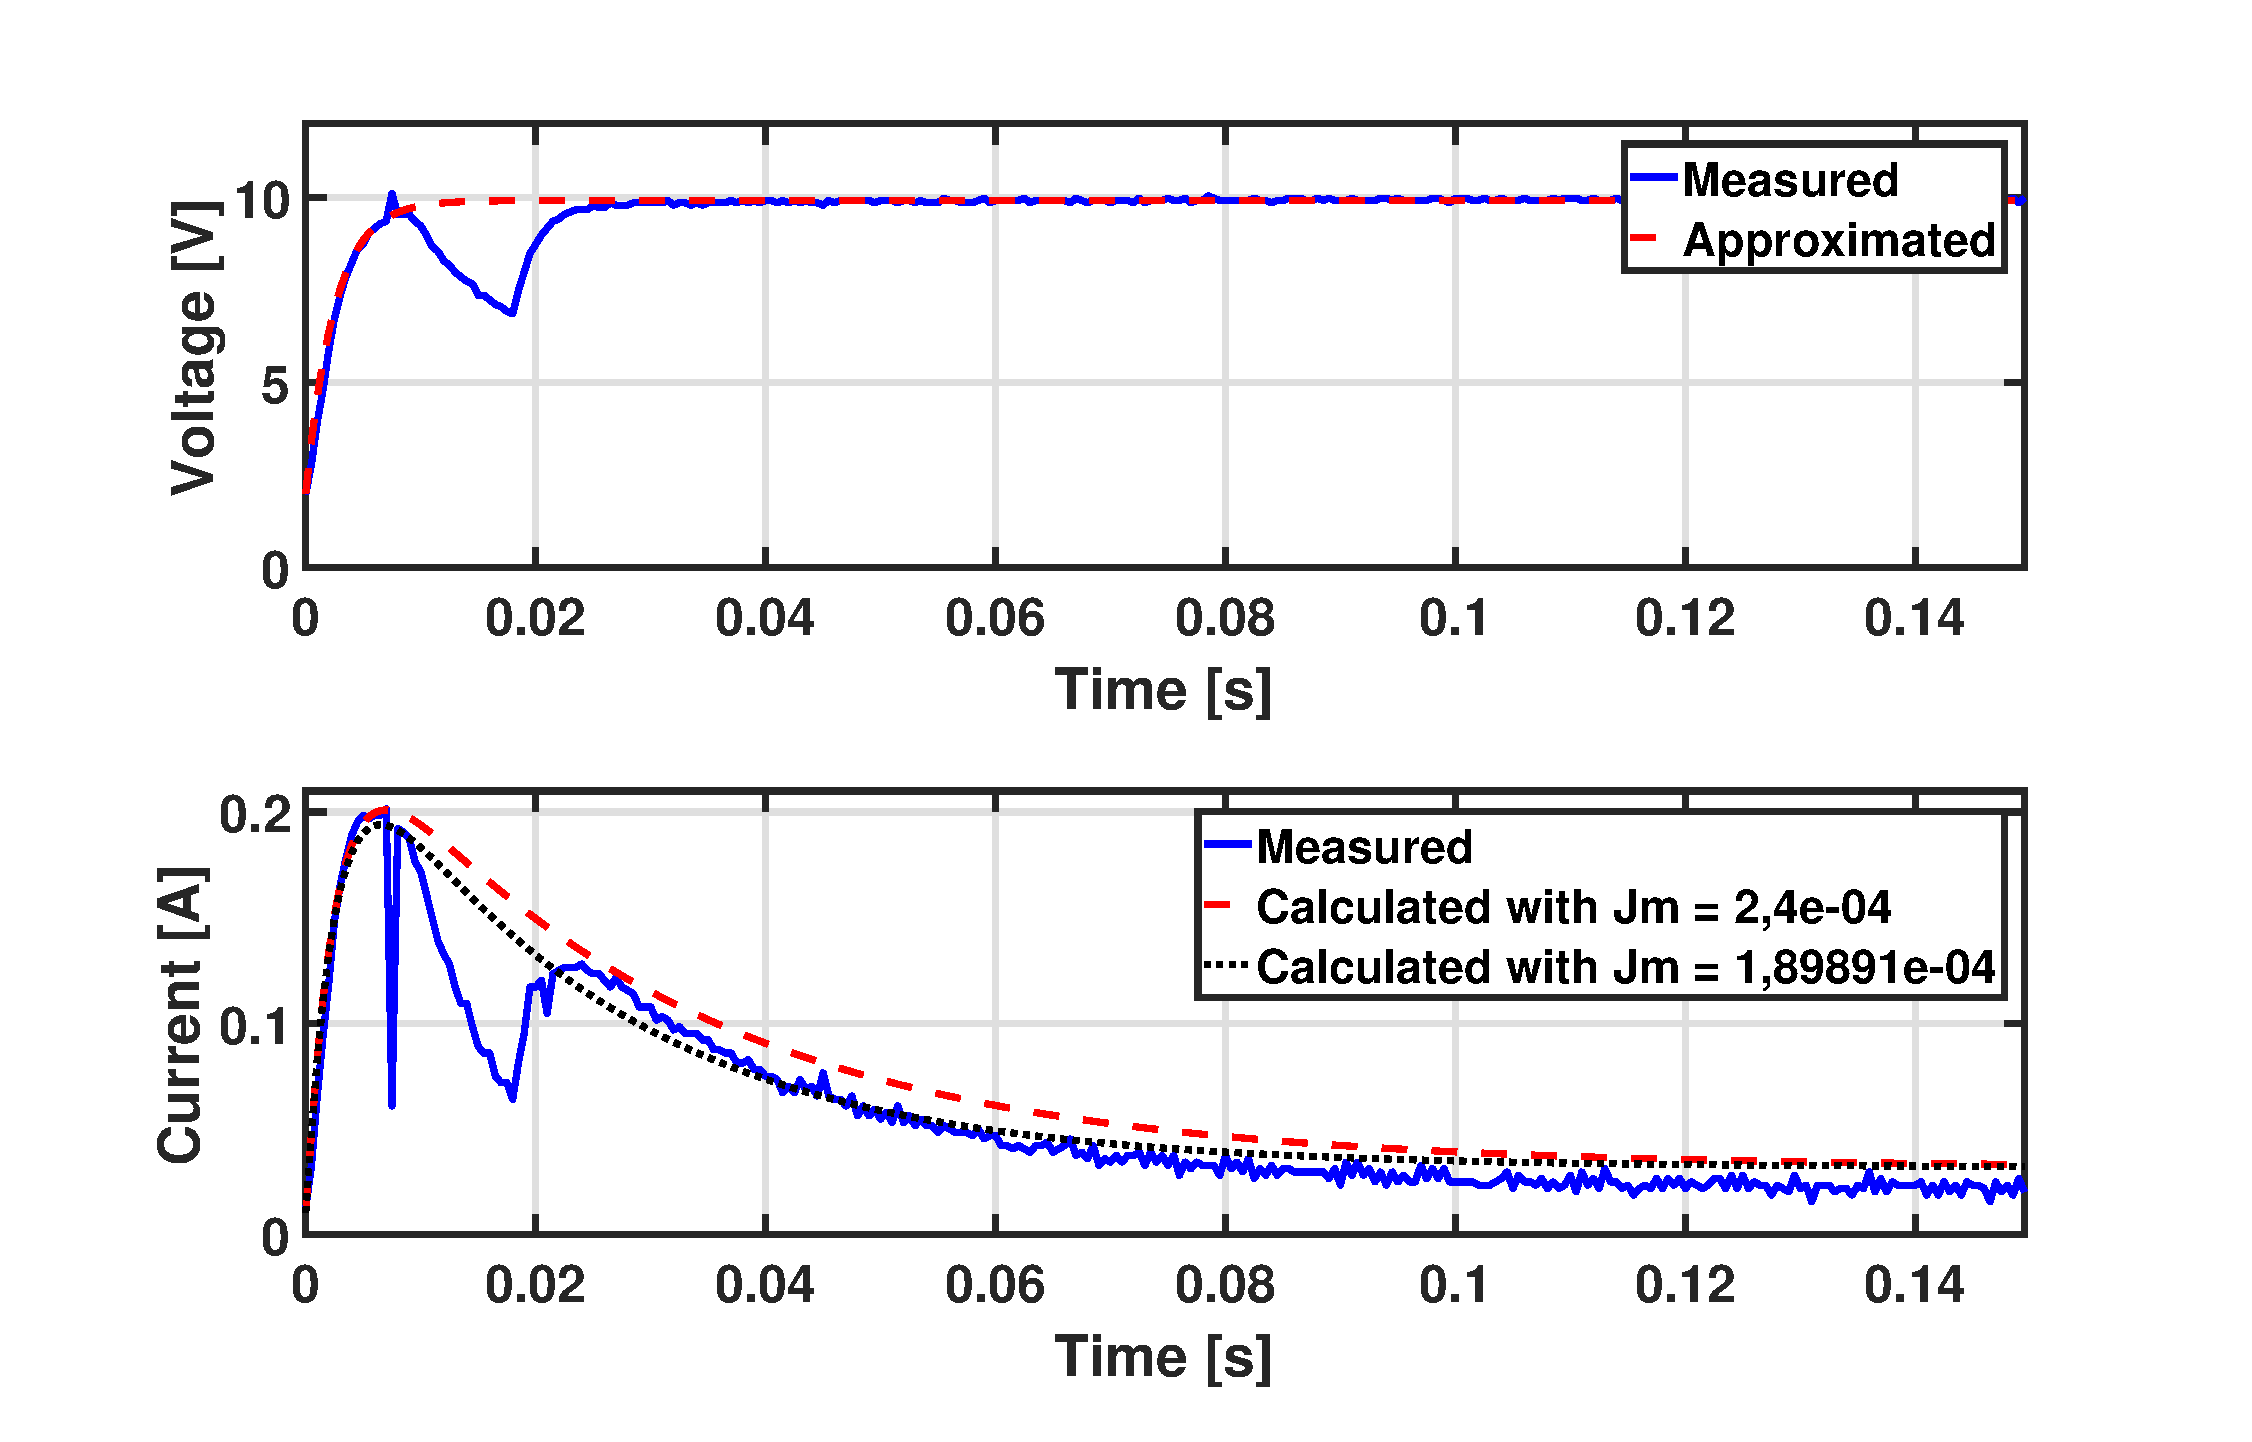
\includegraphics[width=\textwidth]{figures/test/DCMotorMomentOfInertia}
\caption{A graph of the voltage across the DC motor and the corrosponding current in respect to time. The graph contains the measured and calculated curves.}\label{Appendix:fig:DCMotorMomentOfIntertia}
\end{figure}

\section*{Data processing}
Ideally the voltage curve on \autoref{Appendix:fig:DCMotorMomentOfIntertia} would be a sharp step, and the angular velocity in respect to time would be measured. Since the equipment for such measurements is not available, a measurement of the voltage and current is used. A curve fit between the theoretical model and the measurements is made, so that the model has the same dynamic properties (such as rise time, overshoot and settling time) as the measurement.


Two differential equations, Equations \ref{eq:DC-motorElecEq} and \ref{eq:DC-motorMechEqKt}, that describes a model of the DC motor are given in \autoref{sec:DC-motorTechnicalKnowledge}. Since there is no load attached in this test, the two equations can be rewritten as Equations \ref{appendix:eq:DC-motorElecEq} and \ref{appendix:eq:DC-motorMechEqKt}.
\begin{subequations}
\begin{align}
v_{s}(t) &= R_{a}\cdot i_a(t) + \frac{d i_a(t)}{d t}\cdot L_a + K_{e}\cdot\omega_{m}(t) \addunit{\volt}\label{appendix:eq:DC-motorElecEq}\\
J_m \cdot \frac{d \omega_{m}(t)}{d t} &= K_t\cdot i_a(t)- B_m \cdot \omega_{m}(t) \addunit{\newton\metre}\label{appendix:eq:DC-motorMechEqKt}
\end{align}
\end{subequations}

By laplace transformation Equation \ref{appendix:eq:DC-motorEleclaplace} and \ref{appendix:eq:DC-motorMechlaplace} yields.
\begin{subequations}
\begin{align}
V_{s}(s) &= R_{a}\cdot I_a(s) + \left(I_a(s)\cdot s-i_{init}\right) \cdot L_a + K_{e}\cdot\Omega_{m}(s)\label{appendix:eq:DC-motorEleclaplace}\\
J_m \cdot\left( \Omega_m(s)\cdot s - \omega_{init} \right) &= K_t\cdot I_a(s) - B_m \cdot \Omega_{m}(s)\label{appendix:eq:DC-motorMechlaplace}
\end{align}
\end{subequations}

By isolation of $\Omega_m(s)$ in \autoref{appendix:eq:DC-motorMechlaplace}, and insertion into \autoref{appendix:eq:DC-motorEleclaplace}, a relationship between the voltage $V_s(s)$ and the current $I_a(s)$ is shown in \autoref{appendix:eq:DCmotorTs}.

\begin{equation}
I_a(s) = \frac{J_mL_ai_{init}s+B_mL_ai_{init}-J_mK_e\omega_{init}+J_msV_s(s)+B_mV_s(s)}{J_mL_as^2+(B_mL_a+J_mR_a)s+B_mR_a+K_eK_t}\label{appendix:eq:DCmotorTs}
\end{equation}
The initial current $i_{init}$ is measured and the initial angular velocity $\omega_{init}$ is calculated using the initial current, initial voltage and \autoref{appendix:eq:DC-motorElecEq}.
The supply voltage $V_s(s)$ is approximated by as an exponential function and applied to the function which is then inverse laplace transformed to describe current in the time domain.
The moment of inertia $J_m$ is then varied to get the best fit of the dynamic properties of the system. All of this is done through MATLAB using the code shown in \autoref{Appendix:lst:DCMotorJMatlab}.
It is observed that there is a steady state error, which might be due to the approximations made in regards to the motor friction coefficient $B_m$ in \autoref{appendix:TJDCMotorTorqueConstant}.

\lstinputlisting[language = matlab, caption = {Matlab code to approximate the voltage $V_s(s)$ and fit the model of the DC motor to the measurements}, label = {Appendix:lst:DCMotorJMatlab}]{appendixCode/momentOfInertiaCurveFit.m}
The curve fitting gives a value of $J_m = \SI{0.00019}{\newton\metre\second\squared\per\radian}$, it is however seen that the empirically chosen value $J_m = \SI{0.00024}{\newton\metre\second\squared\per\radian}$ has a better fitting rise time, overshoot and settling time compared to the measured data.

\section*{Conclusion}
The result for the test and calculation is that the moment of inertia of the DC motors rotational body is $J_m = \SI{0.00024}{\newton\metre\second\squared\per\radian}$.